% MFCCs are modeled with a Gaussian Mixture Model, which is a parametric probability density
% function represented as a weighted sum of Gaussian component densities. GMMs are often
% used in biometric systems, specially in speaker recognition systems, due to their
% capability of representing a large class of sample distributions. One of the powerful
% attributes of the GMM is its ability to form smooth aproximations to arbitrarily shaped
% densities \cite{gmm_reynolds}.

% The densitiy function of a GMM is defined as:

% \begin{equation}
% 	p(x) = \sum_{k=1}^{K}\pi_{k} \mathcal{N}(x|\mu_{k},\,\Sigma_{k})
% \end{equation}

% Each Gaussian density $\mathcal{N}(x|\mu_{k},\,\Sigma_{k})$ is called a component of the mixture
% and has its own mean $\mu_{k}$ and variance $\Sigma_{k}$. The parameters $\pi_{k}$ are called
% mixing coefficients and they can be thought of as the prior probability of picking the $k^{th}$
% component \cite{gmm_bishop}.

% Each Gaussian component is determined by the formula:

% \begin{equation}
% 	\mathcal{N}(x|\mu_{k},\,\Sigma_{k}) = \frac{1}{(2\pi)^{(D/2)}|\Sigma|^{1/2}} exp \big\{ -\frac{1}{2}(x-\mu)^{T}\Sigma^{-1}(x-\mu)\}
% \end{equation}

% Where $D$ is the dimension of the features space (39 MFCCs in this case), the $D$-dimensional
% vector $\mu$ is the mean, the $DxD$ matrix $\Sigma$ is called the covariance and $|\Sigma|$
% denotes the determinant of $\Sigma$.

% \subsection{Expectation Maximization Algorithm}

% Given the training vectors, the objective is to estimate the parameters $\lambda$ of the GMM
% that in some sense best matches the distribution of the data. The aim of the estimation is
% to find the model parameters which maximize the likelihood of the given training data. For a
% sequence of $N$ training vectors $X=\{x_{1}, x_{2}, \dotsc x_{N}\}$ the GMM likelihood
% (assuming independence between vectors) can be written as:

% \begin{equation}
% 	\label{eq:likelihoodGMM}
% 	p(X|\lambda) = \prod_{n=1}^{N}p(x_{n}|\lambda)
% \end{equation}

% The parameters $\lambda$ that maximizes \ref{eq:likelihoodGMM} are obtained by using an iterative
% algorithm called Expectation Maximization. The basic idea of the EM algorithm is,
% beginning with an initial model $\lambda$ (i.e random initialized), estimate a new model
% $\bar{\lambda}$ such that $p(X|\bar{\lambda}) \geq p(X|\lambda)$. The new model then becomes
% the initial model for the next iteration and the process is repeated until some convergence
% model is reached.

% Each iteration involves two steps that give the algorithm its name. Given the training vectors
% $X=\{x_{1}, x_{2} \dotsc x_{N}\}$, the first step is the \emph{Expectation} step,
% where the posterior probabilities $P(k|x_{n})$ are computed.
% These posteriors represents the \emph{responsibility} that component $k$ takes for
% 'explaining' the observation $x_{n}$.

% \begin{equation}
% 	P(k|x_{n}) = \frac{\pi_{k} \mathcal{N}(x_{n}|\mu_{k},\,\Sigma_{k})}{\sum_{j=1}^{K}\pi_{k} \mathcal{N}(x_{n}|\mu_{j},\,\Sigma_{j})}
% 	\label{eq:expectationStep}
% \end{equation}

% During the Maximization step, the parameters are re-estimated using the current responsibilities:

% \begin{equation}
% 	\pi_{k}^{new} = \frac{\sum_{n=1}^{N}P(k|x_{n})}{N}
% \end{equation}

% \begin{equation}
% 	\label{eq:gmmExpectedValue}
% 	\mu_{k}^{new} = \frac{1}{N_{k}}\sum_{n=1}^{N}P(k|x_{n})x_{n}
% \end{equation}

% \begin{equation}
% 	\label{eq:gmmVariance}
% 	\Sigma_{k}^{new} = \frac{1}{N_{k}}\sum_{n=1}^{N}P(k|x_{n})(x_{n} - \mu_{k}^{new})(x_{n} - \mu_{k}^{new})^{T}
% \end{equation}

% where $N_{k}$ can be interpreted as the effective number of points assigned to cluster $k$
% and is defined as:

% \begin{equation}
% 	\label{eq:gmmNk}
% 	N_{k} = \sum_{n=1}^{N}P(k|x_{n})
% \end{equation}

% After the Maximization step, the log likelihood of the new model is evaluated and the convergence
% criterion is evaluated for either the parameters or the log likelihood:

% \begin{equation}
% 	ln \ p(X|\mu, \Sigma, \pi) = \sum_{n=1}^{N}ln\Big\{\sum_{k=1}^{K}\pi_{k}\mathcal{N}(x_{n}|\mu_{k},\,\Sigma_{k})\Big\}
% \end{equation}


% If the convergence criterion is not satisfied, the algorithm returns to \ref{eq:expectationStep}
% to start a new iteration of the Expectation and Maximization steps.

% \subsection{\textit{Universal Background Model} Adaptation}

% % A \textit{GMM} model trained using \textit{MFCCs} as input features is the chosen classifier for
% % the first experiment of the current work. The classifiers for the are trained with features
% In the present work, as in the previous works of the current line of investigation
% \cite{detection_phone_level_mispronunciation_learning, main}, the \textit{GMMs} are derived
% by using a techinque called \textit{GMM-UBM} \textit{Universal Background Model} \cite{ubm_adaptation}.

% The \textit{UBM} is a large class-independent \textit{GMM} intended to represent the whole possible
% distribution of the features. In a \textit{GMM-UBM} system, the
% \textit{GMM} is derived by adapting the parameters of the \textit{UBM} using the particular
% instances according to the custom desired model and a form of
% \textit{Maximum a Posteriori} (\textit{MAP}) estimation. This provides a tighter coupling
% between the particular models and the \textit{UBM} that produces better performance than
% using decoupled models, and it can be specially useful for the models that has a small number
% of training instances. The method described in \cite{ubm_adaptation} involves adapting weight,
% mean and variance of each mixture, though in the current work only weights and means are adapted
% because of the limited size of the dataset.

% The adaptation process, like the \textit{EM} algorithm, is a two step estimation process.
% The first step is identical to the expectation step of the \textit{EM} algorithm, where estimates
% of the sufficient statistics of the training data are computed for each mixture in the
% \textit{UBM}. For the second step of the adaptation, however, these new sufficient statistics
% estimates are then combined with the old sufficient statistics from the \textit{UBM}
% mixture parameters using a parameter-dependent mixing coefficient. The
% mixing coefficient is designed so that mixtures with high counts of data
% from the adaptation data rely more on the new
% sufficient statistics for final parameter estimation and mixtures with low counts of data
% from the adaptation data rely more on the old sufficient statistics for final parameter
% estimation.

% Given a \textit{UBM} and the adaptation vectors $X=\{x_{1}, x_{2} \dotsc x_{N}\}$, the first step
% in the adaptation process is to compute the posterior probabilities representing the
% \textit{responsibility} that the mixture $k, \ 1 \leq k \leq K$ of the \textit{UBM}
% takes for 'explaining' each observation
% (as in the first step of the \textit{EM} \ref{eq:expectationStep}):

% \begin{equation}
% P(k|x_{n}) = \frac{\pi_{k}p_{k}(x_{n})}{\sum_{j=1}^{K}\pi_{j}p_{j}(x_{n})}
% \end{equation}

% where $p_{k}(x_{n}), \ 1 \leq k \leq K$ is the likelihood of the observation $x_{n}$ given the
% mixture $k$ of the \textit{UBM}.

% Posterior probabilities are then used to compute sufficient statistics for the weight, mean
% and variance parameters, as in the equations \ref{eq:gmmNk}, \ref{eq:gmmExpectedValue} and \ref{eq:gmmVariance} respectively of the \textit{EM expectation step}:

% \begin{equation}
% 	N_{k} = \sum_{n=1}^{N}P(k|x_{n})
% \end{equation}

% \begin{equation}
% 	E_{k}(x) = \frac{1}{N_{k}}\sum_{n=1}^{N}P(k|x_{n})x_{n}
% \end{equation}

% \begin{equation}
% 	E_{k}(x^{2}) = \frac{1}{N_{k}}\sum_{n=1}^{N}P(k|x_{n})x_{n}^{2}
% \end{equation}

% Finally, these new sufficient statistics from the training data are used to update the old
% suficient statistics from mixture $k$ to create the adapted parameters for mixture $k$ with
% the equations:

% \begin{equation}
% 	\pi_{k}^{new} = [\alpha_{k} N_{k} / N + (1-\alpha_{k}) \pi_{k}]\gamma
% \end{equation}

% \begin{equation}
% 	\mu_{k}^{new}	= \alpha_{k} E_{k}(x) + (1-\alpha_{k})\mu_{k}
% \end{equation}

% \begin{equation}
% 	\Sigma_{k}^{new} = \alpha_{k} E_{k}(x^{2}) + (1-\alpha_{k})(\Sigma_{k}^{2} + \mu_{k}^{2}) - (\mu_{k}^{new})^{2}
% \end{equation}

% The scale factor $\gamma$ is computed over all adapted mixture weights to ensure they sum to unity.
% $\alpha_{k}$ is the adaptation coefficient that controls the balance between old and new
% estimates, and is defined as:

% \begin{equation}
% 	\alpha_{k} = \frac{N_{k}}{N_{k} + r}
% \end{equation}

% where $r$ is the relevance factor input parameter. This way, if a mixture component has a low
% probabilistic count $N_{k}$ of the new data, then $\alpha_{k} \to 0$ causing the deemphasis
% of the new (potentially undertrained) parameters and the emphasis of the old (better trained)
% parameters. On the other hand, for mixture components with high probabilistic counts,
% $\alpha_{k} \to 1$ incresaing the emphasis on the new adapted parameters.

% \begin{figure}[H]
% 	\centering
% 	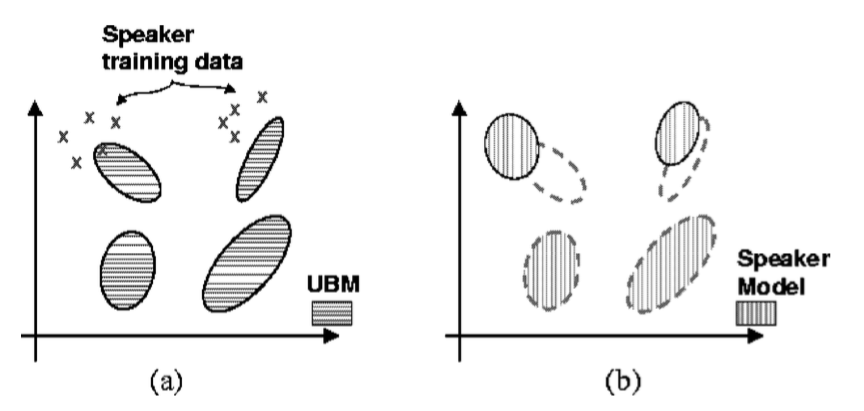
\includegraphics[width=0.8\textwidth]{files/figures/method/gmm-adaptation}
% 	\caption{Taken from \cite{ubm_adaptation}. Example
% 	of an adaptation of mixtures of an speaker-independent \textit{UBM} using data of an
% 	individual speaker. (a) The training vectors (x's) are probabilistically mapped into
% 	the \textit{UBM} mixtures. (b) The adapted mixture parameters are derived using the
% 	statistics of the new data and the previous \textit{UBM} mixture parameters. The
% 	adaptation is data-dependent, so each mixture is adapted by different amounts.}
% \end{figure}

